\documentclass{beamer}
\usepackage{notation}
\usepackage{forloop}

\usetheme{metropolis}           % Use metropolis theme
\title{Gaussian Processes}
\date{\today}
\author{Nipun Batra}
\institute{IIT Gandhinagar}
\begin{document}
  \maketitle
  
  
  
\section{Gaussian Distribution}
  \begin{frame}{1d Gaussian Scatter Plot}
    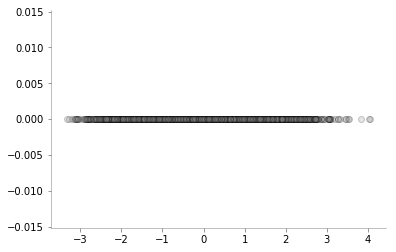
\includegraphics[width=\linewidth,height=\textheight,keepaspectratio]{gp/1d-gp}
  \end{frame}

  \begin{frame}{1d Gaussian Histogram}
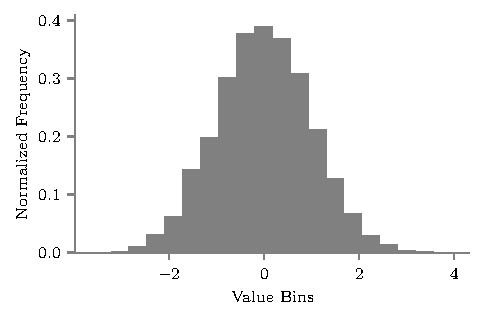
\includegraphics[width=\linewidth,height=\textheight,keepaspectratio]{gp/1d-gp-hist}
\end{frame}

  \begin{frame}{Varying 1d Gaussian Variance}
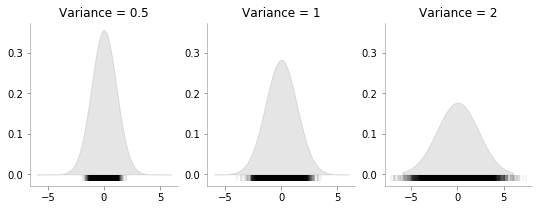
\includegraphics[width=\linewidth,height=\textheight,keepaspectratio]{gp/1d-gp-kde2}\end{frame}

\begin{frame}{Bi-variate Gaussian}
$$
\begin{pmatrix}
X_1 \\
X_2
\end{pmatrix}  \sim \mathcal{N} \left( \begin{pmatrix}
\mu_1 \\
\mu_2
\end{pmatrix} , \begin{pmatrix}
a &\rho \\
\rho & b
\end{pmatrix} \right)
$$
\end{frame}

\begin{frame}{Sampling Bi-variate Gaussian - 1}
\begin{center}
	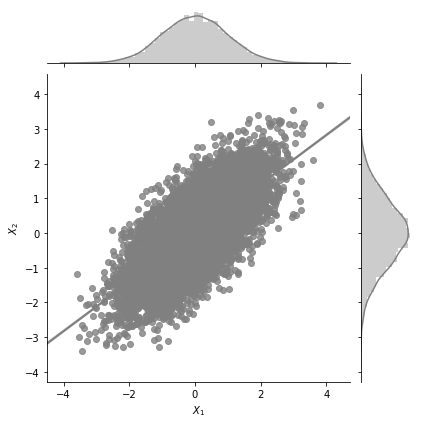
\includegraphics[height=\textheight -10pt ,keepaspectratio]{gp/2d-gp}
\end{center}
\end{frame}


\begin{frame}{Sampling Bi-variate Gaussian - 2}
	\begin{center}
		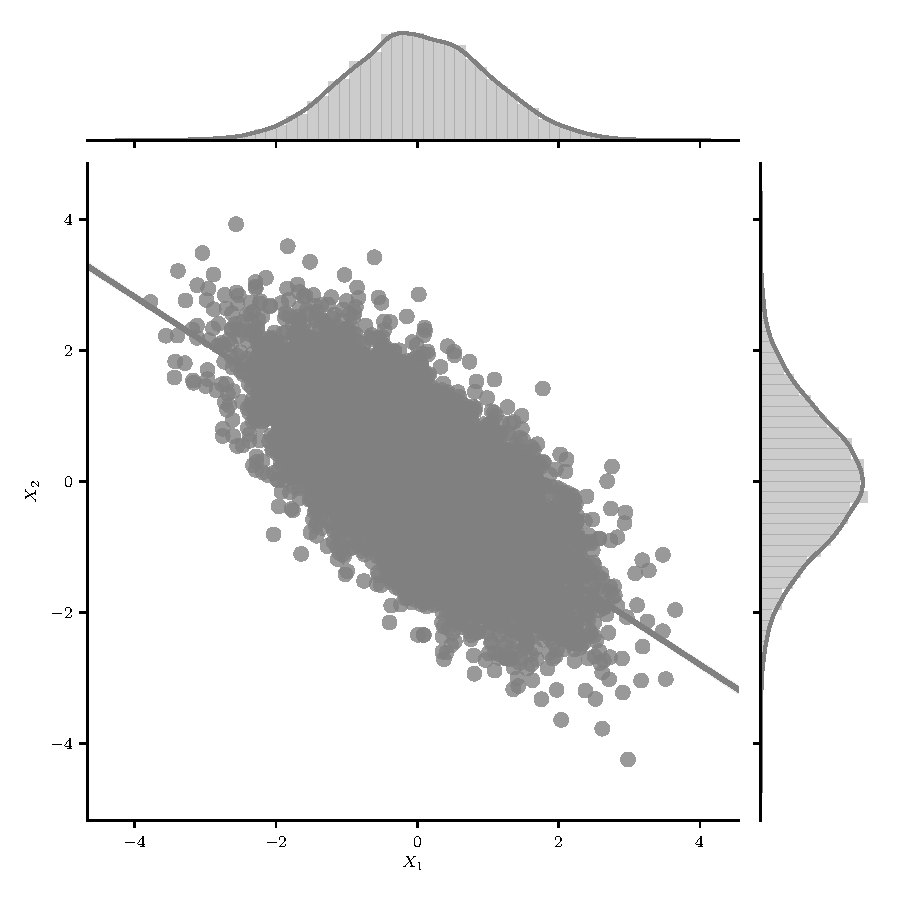
\includegraphics[height=\textheight -10pt ,keepaspectratio]{gp/2d-gp2}
	\end{center}
\end{frame}

\begin{frame}{Sampling Bi-variate Gaussian - 3}
	\begin{center}
		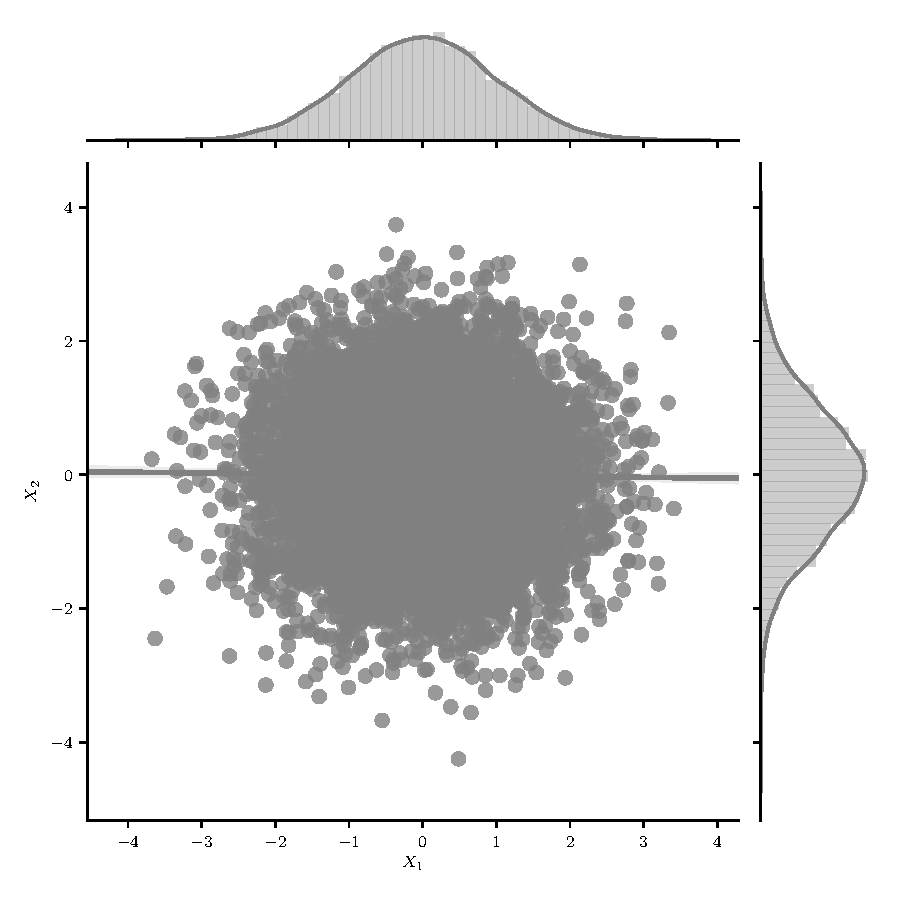
\includegraphics[height=\textheight -10pt ,keepaspectratio]{gp/2d-gp3}
	\end{center}
\end{frame}

\begin{frame}{Surface Plots Bi-variate Gaussian - 1}
	\begin{center}
		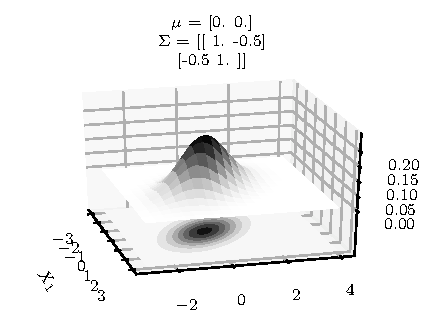
\includegraphics[height=\textheight -10pt ,keepaspectratio]{gp/2dgp3d}
	\end{center}
\end{frame}

\begin{frame}{Surface Plots Sampling Bi-variate Gaussian - 2}
	\begin{center}
		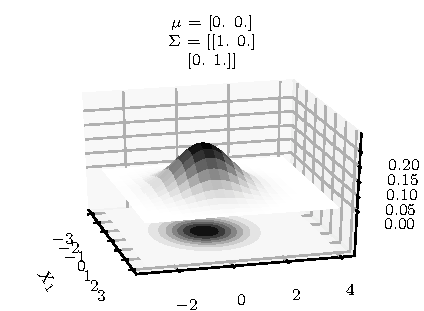
\includegraphics[height=\textheight -10pt ,keepaspectratio]{gp/2dgp3d2}
	\end{center}
\end{frame}

\section{Visualizing samples from 2d Gaussian}

% for cov
\newcounter{iter}
\forloop{iter}{1}{\value{iter} < 6}%
{%
	\begin{frame}{Cov = 0.1 | Random State - \theiter}
		\includegraphics[width=\linewidth,height=\textheight,keepaspectratio]{gp/0.1/\theiter}
	\end{frame}
}
% for cov
\forloop{iter}{1}{\value{iter} < 6}%
{%
	\begin{frame}{Cov = 0.7 | Random State - \theiter}
		\includegraphics[width=\linewidth,height=\textheight,keepaspectratio]{gp/0.7/\theiter}
	\end{frame}
}

\section{Conditional Bi-variate Distribution}

\begin{frame}{Conditional Bi-variate Distribution}
$$
\begin{pmatrix}
	X_1 \\
	X_2
\end{pmatrix}  \sim \mathcal{N} \left( \begin{pmatrix}
	0 \\
	0
\end{pmatrix} , \begin{pmatrix}
	1 & \rho \\
	\rho & 1
\end{pmatrix} \right)
$$

The conditional expectation of $X_2$ given $X_1$ is: $\operatorname{E}(X_2 \mid X_1=x_1)= \rho x_1$

and the conditional variance is: $\operatorname{var}(X_2 \mid X_1 = x_1) = 1-\rho^2$
\end{frame}

% for cov
\forloop{iter}{1}{\value{iter} < 6}%
{%
	\begin{frame}{Conditional bi-variate | Cov = 0.1 | Random State - \theiter}
		\includegraphics[width=\linewidth,height=\textheight,keepaspectratio]{gp/conditional/0.1/\theiter}
	\end{frame}
}

% for cov
\forloop{iter}{1}{\value{iter} < 6}%
{%
	\begin{frame}{Conditional bi-variate | Cov = 0.7 | Random State - \theiter}
		\includegraphics[width=\linewidth,height=\textheight,keepaspectratio]{gp/conditional/0.7/\theiter}
	\end{frame}
}

\section{5D Multi-variate}

% for cov
\forloop{iter}{1}{\value{iter} < 6}%
{%
	\begin{frame}{Multi-variate Gaussian Sample | Random State - \theiter}
		\begin{center}
			\includegraphics[width=\linewidth, height=\textheight -120pt ,keepaspectratio]{gp/5d/\theiter}
		\end{center}
		From the visualisation above we can see that:
		\begin{itemize}
			\item Since $X_1$ and $X_2$ are highly correlated, they move up and down together
			\item but, $X_1$ and $X_5$ have low correlation, thus, they can seem to wiggle almost independently of each other.
		\end{itemize}
	\end{frame}
}

\begin{frame}{Cholesky Decompostion I}
\begin{align*}
\vecMat{A} = \vecMat{L}\vecMat{L}^T
\end{align*}
where $\vecMat{L}$ is a real lower triangular matrix.


We can thus re-write the posterior mean and covariance as:

\begin{align*}
p(\vecMat{y_*}|\vecMat{X_*}, \vecMat{X}, \vecMat{y}) \sim \distrib{N}{\mu'}{\Sigma'} \\
\vecMat{K} = \vecMat{LL}^T \\
\end{align*}
\end{frame}

\begin{frame}{Cholesky Decomposition II}
\begin{align*}
\vecMat{\alpha} = \vecMat{K}^{-1}(\vecMat{x}-\vecMat{\mu}) \\
or, \vecMat{\alpha} = {\vecMat{LL}^T}^{-1}(\vecMat{x}-\vecMat{\mu}) \\
or, \vecMat{\alpha} = \vecMat{L}^{-T}\vecMat{L}^{-1}(\vecMat{x}-\vecMat{\mu}) \\
Let, \vecMat{K}^{-1}(\vecMat{x}-\vecMat{\mu}) = \vecMat{\beta} \\
Thus, \vecMat{L}^{-T}\vecMat{L}^{-1}(\vecMat{x}-\vecMat{\mu}) = \vecMat{\beta} \\
Let, \vecMat{L}^{-1}(\vecMat{x}-\vecMat{\mu}) = \vecMat{\gamma}\\
Thus, \vecMat{L}\vecMat{\gamma} = \vecMat{x}-\vecMat{\mu} \\
Thus, \vecMat{\gamma} = \vecMat{L} \setminus (\vecMat{x}-\vecMat{\mu})\\\
Thus, \vecMat{\alpha} = \vecMat{L}^{T} \setminus (\vecMat{L} \setminus (\vecMat{x}-\vecMat{\mu}))
\end{align*}

\end{frame}
\end{document}